\section{Prompt Engineering}
\label{sec:pe}
%
\begin{frame}[t] \frametitle{\emph{Prompt Engineering}}
\framesubtitle{Definizione}
{\small
\onslide<1->
    \begin{minipage}[t]{\textwidth}
        \vspace*{-.5cm}
        \begin{figure}
            \centering
            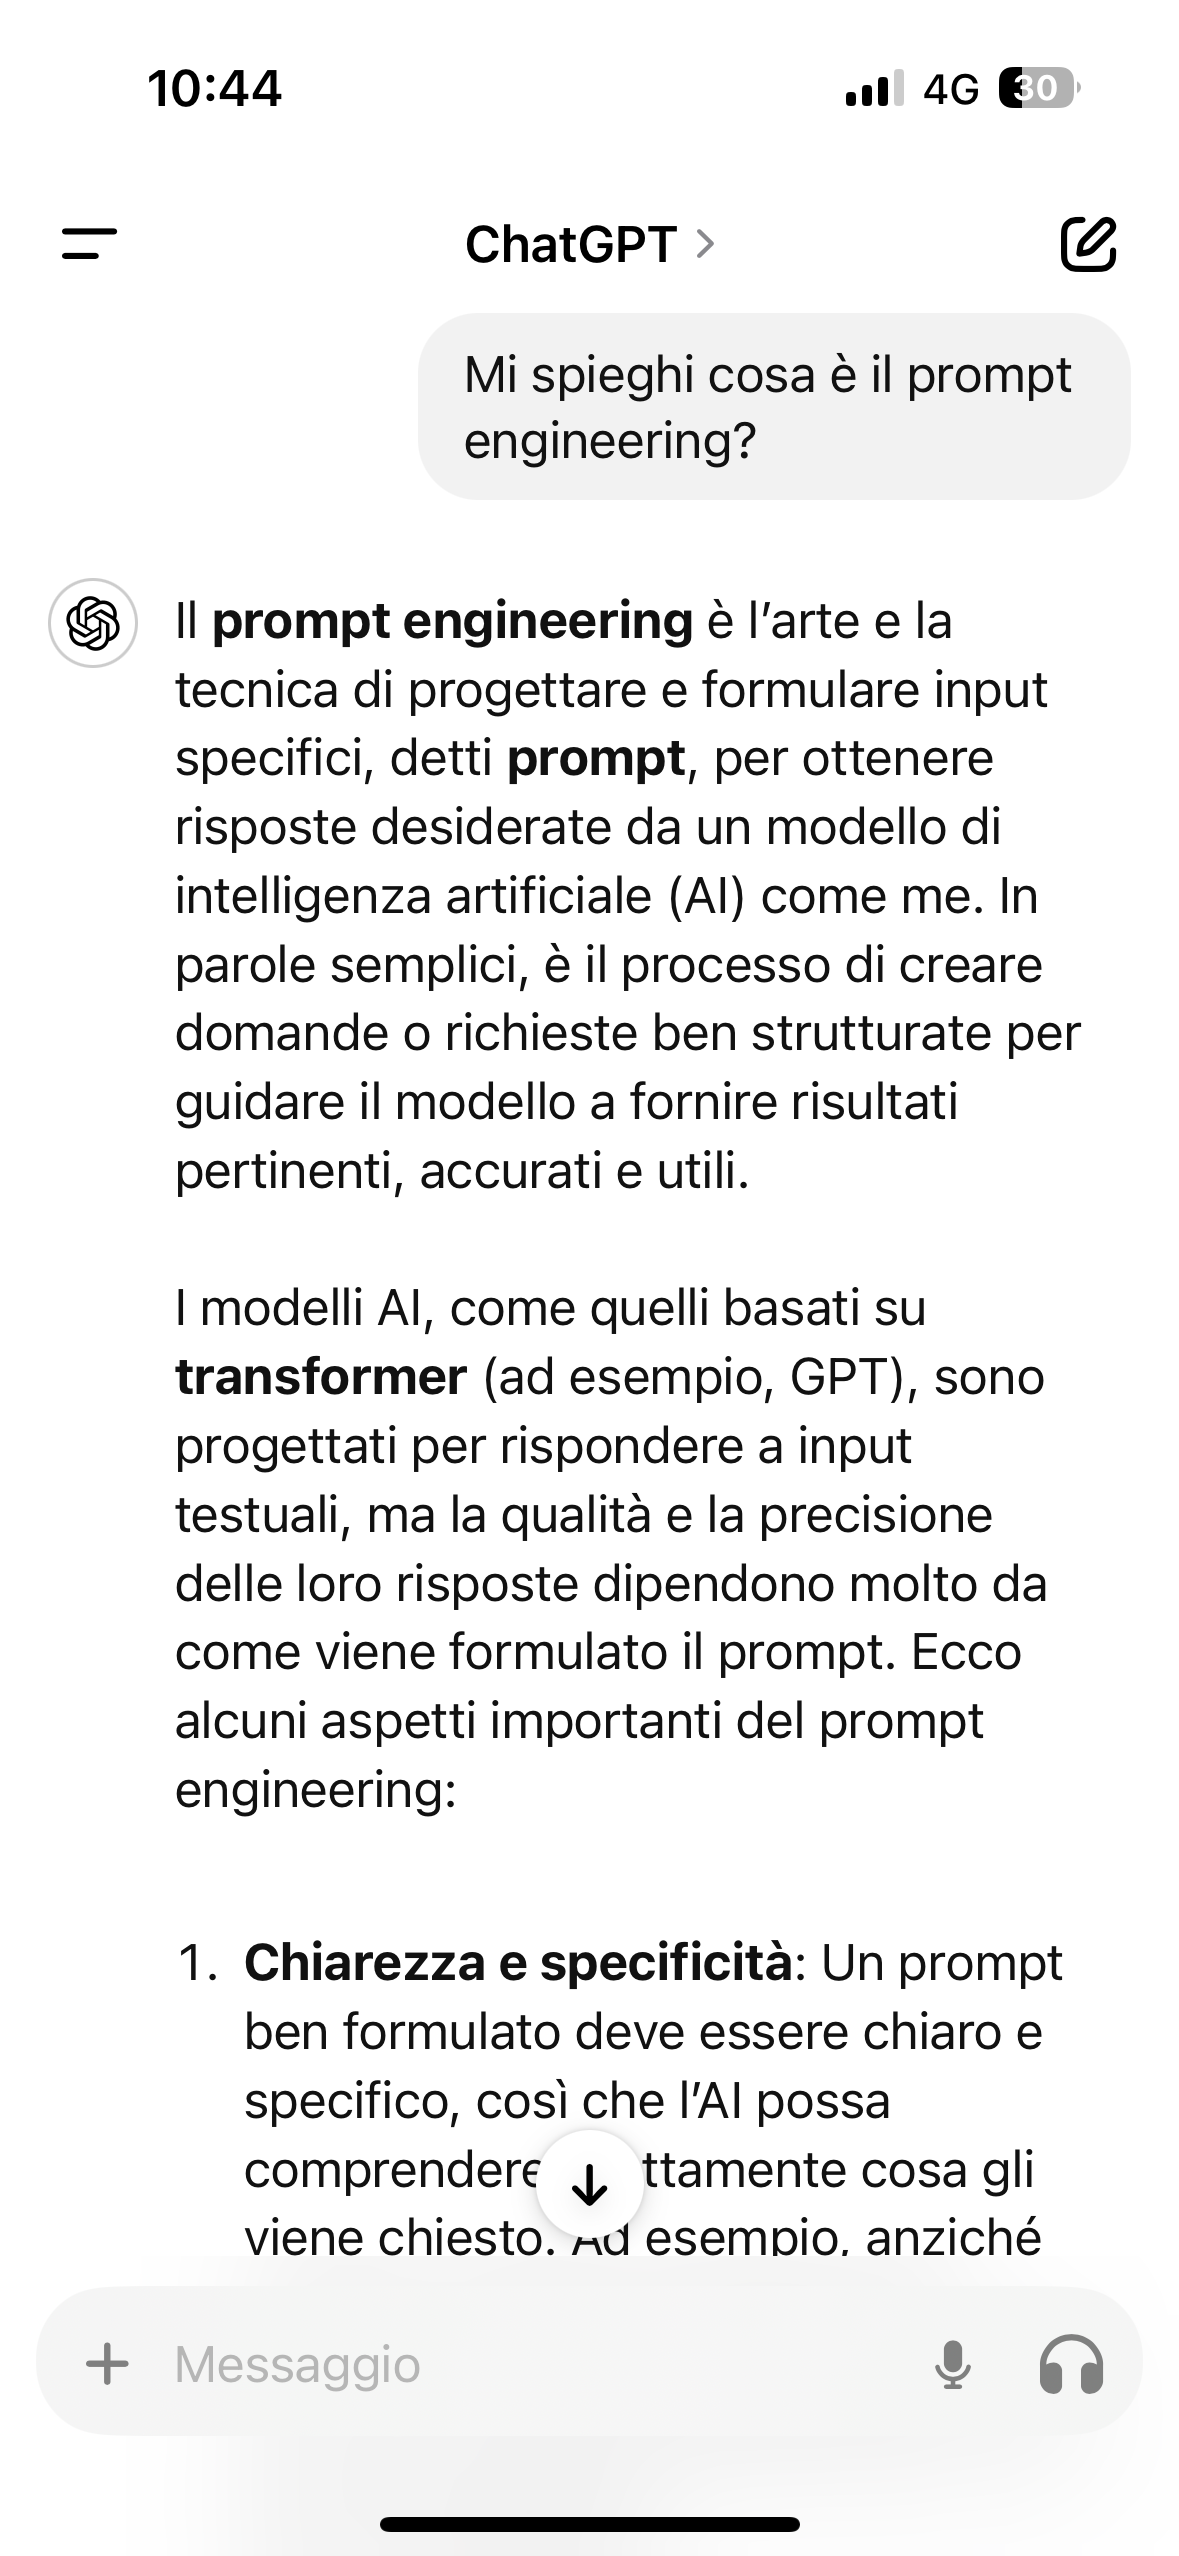
\includegraphics[width=.25\textwidth]{img/PE-1.PNG}
            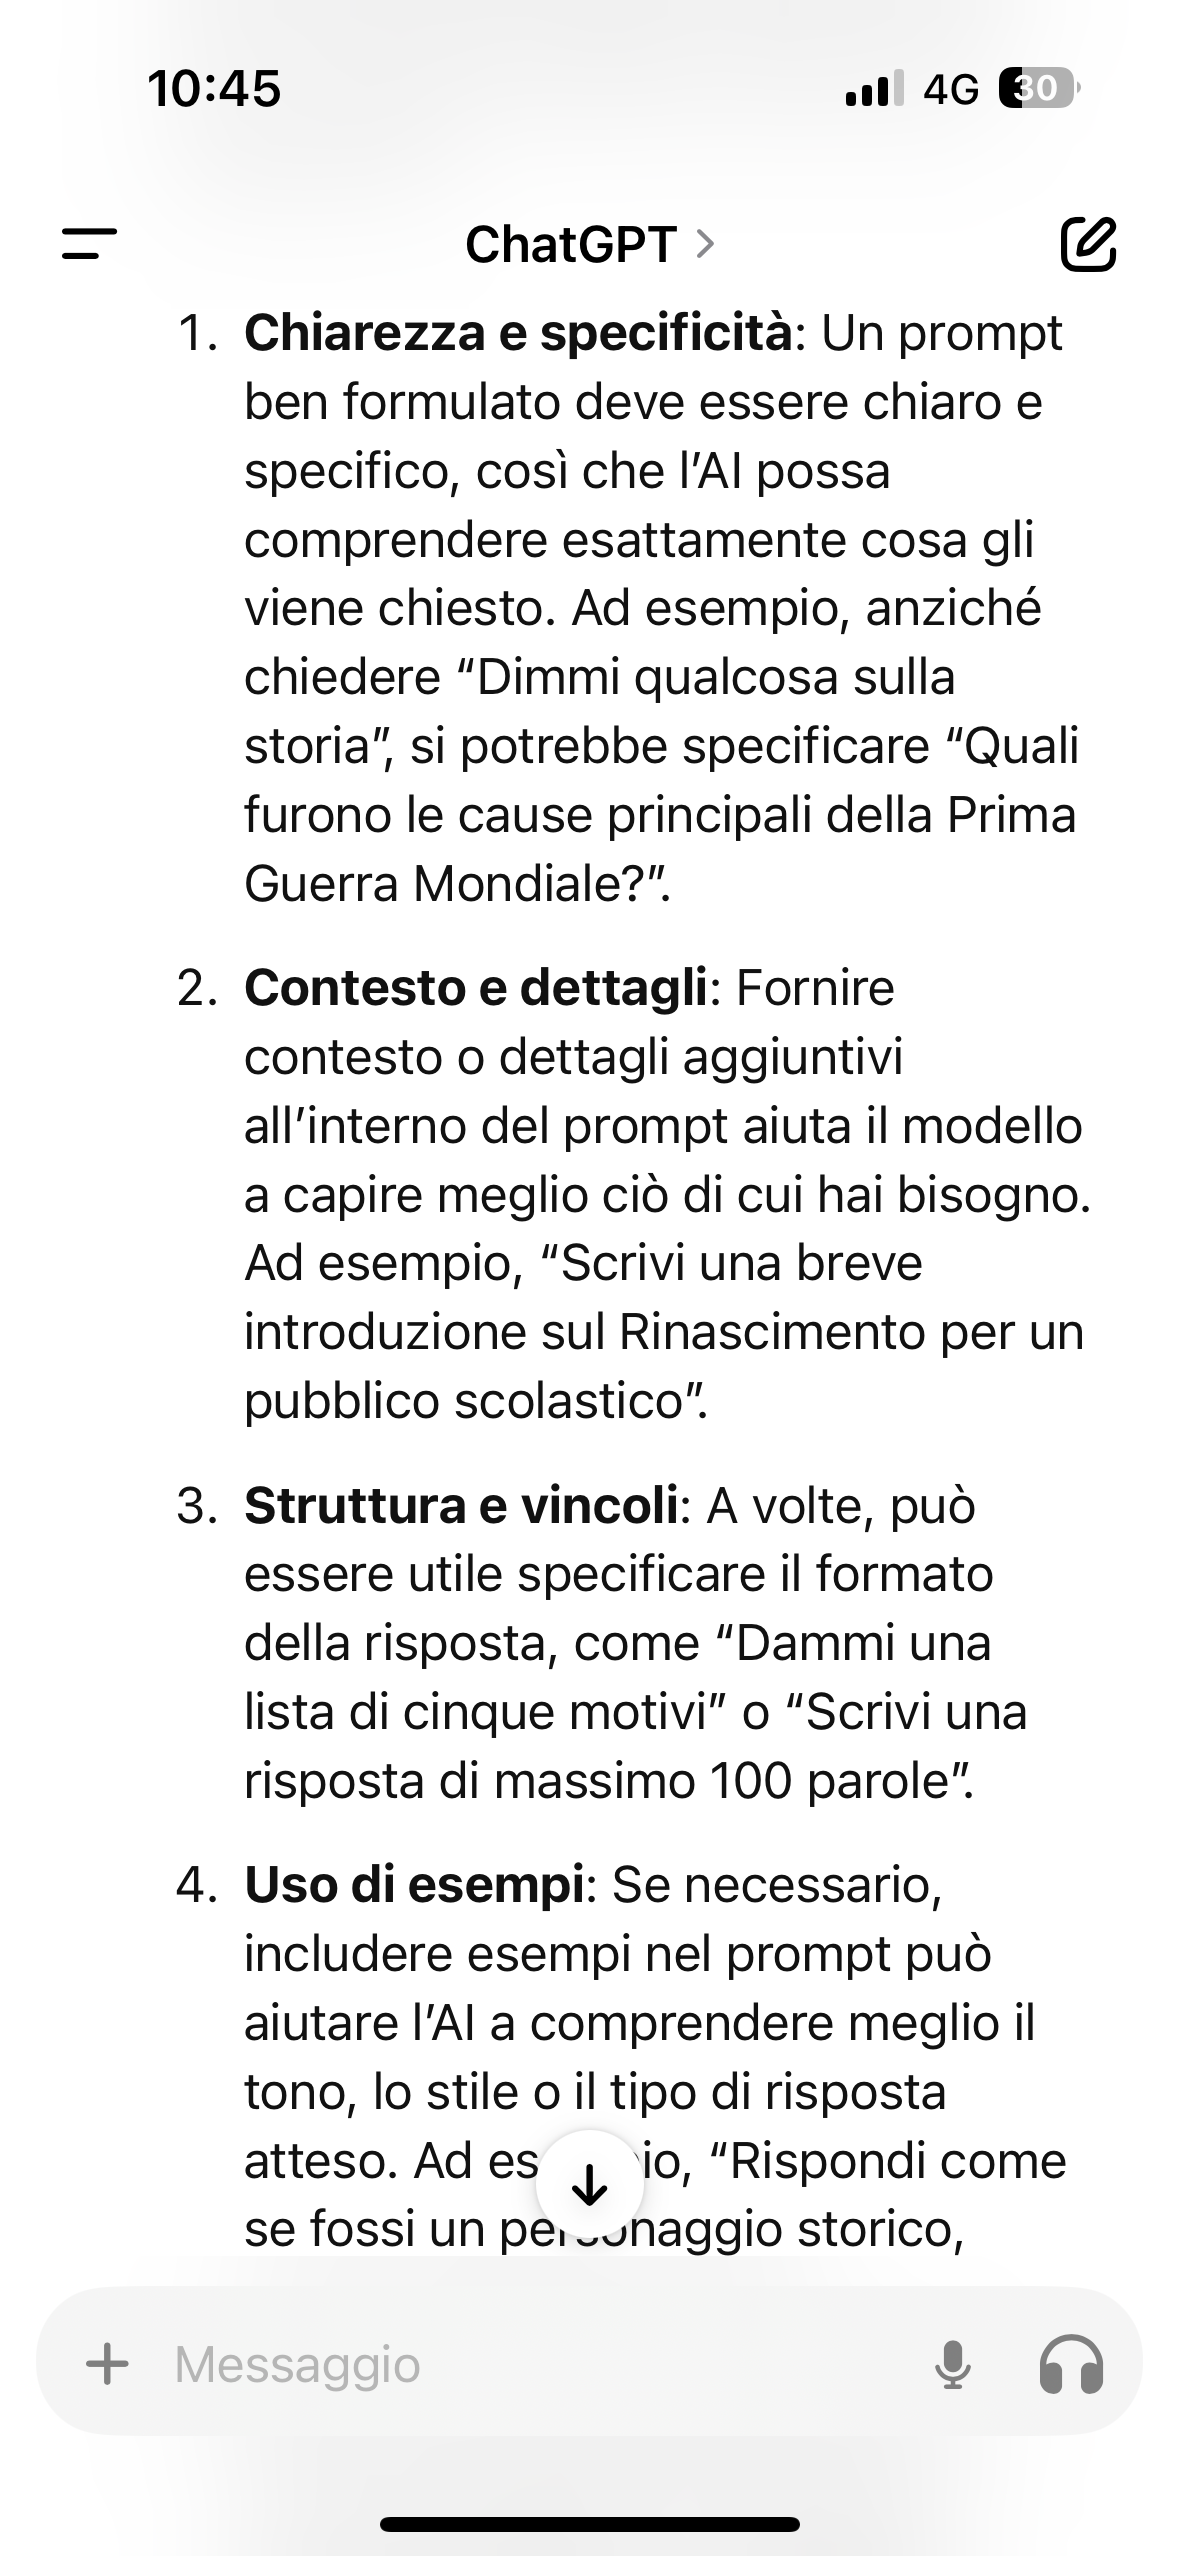
\includegraphics[width=.25\textwidth]{img/PE-2.PNG}
            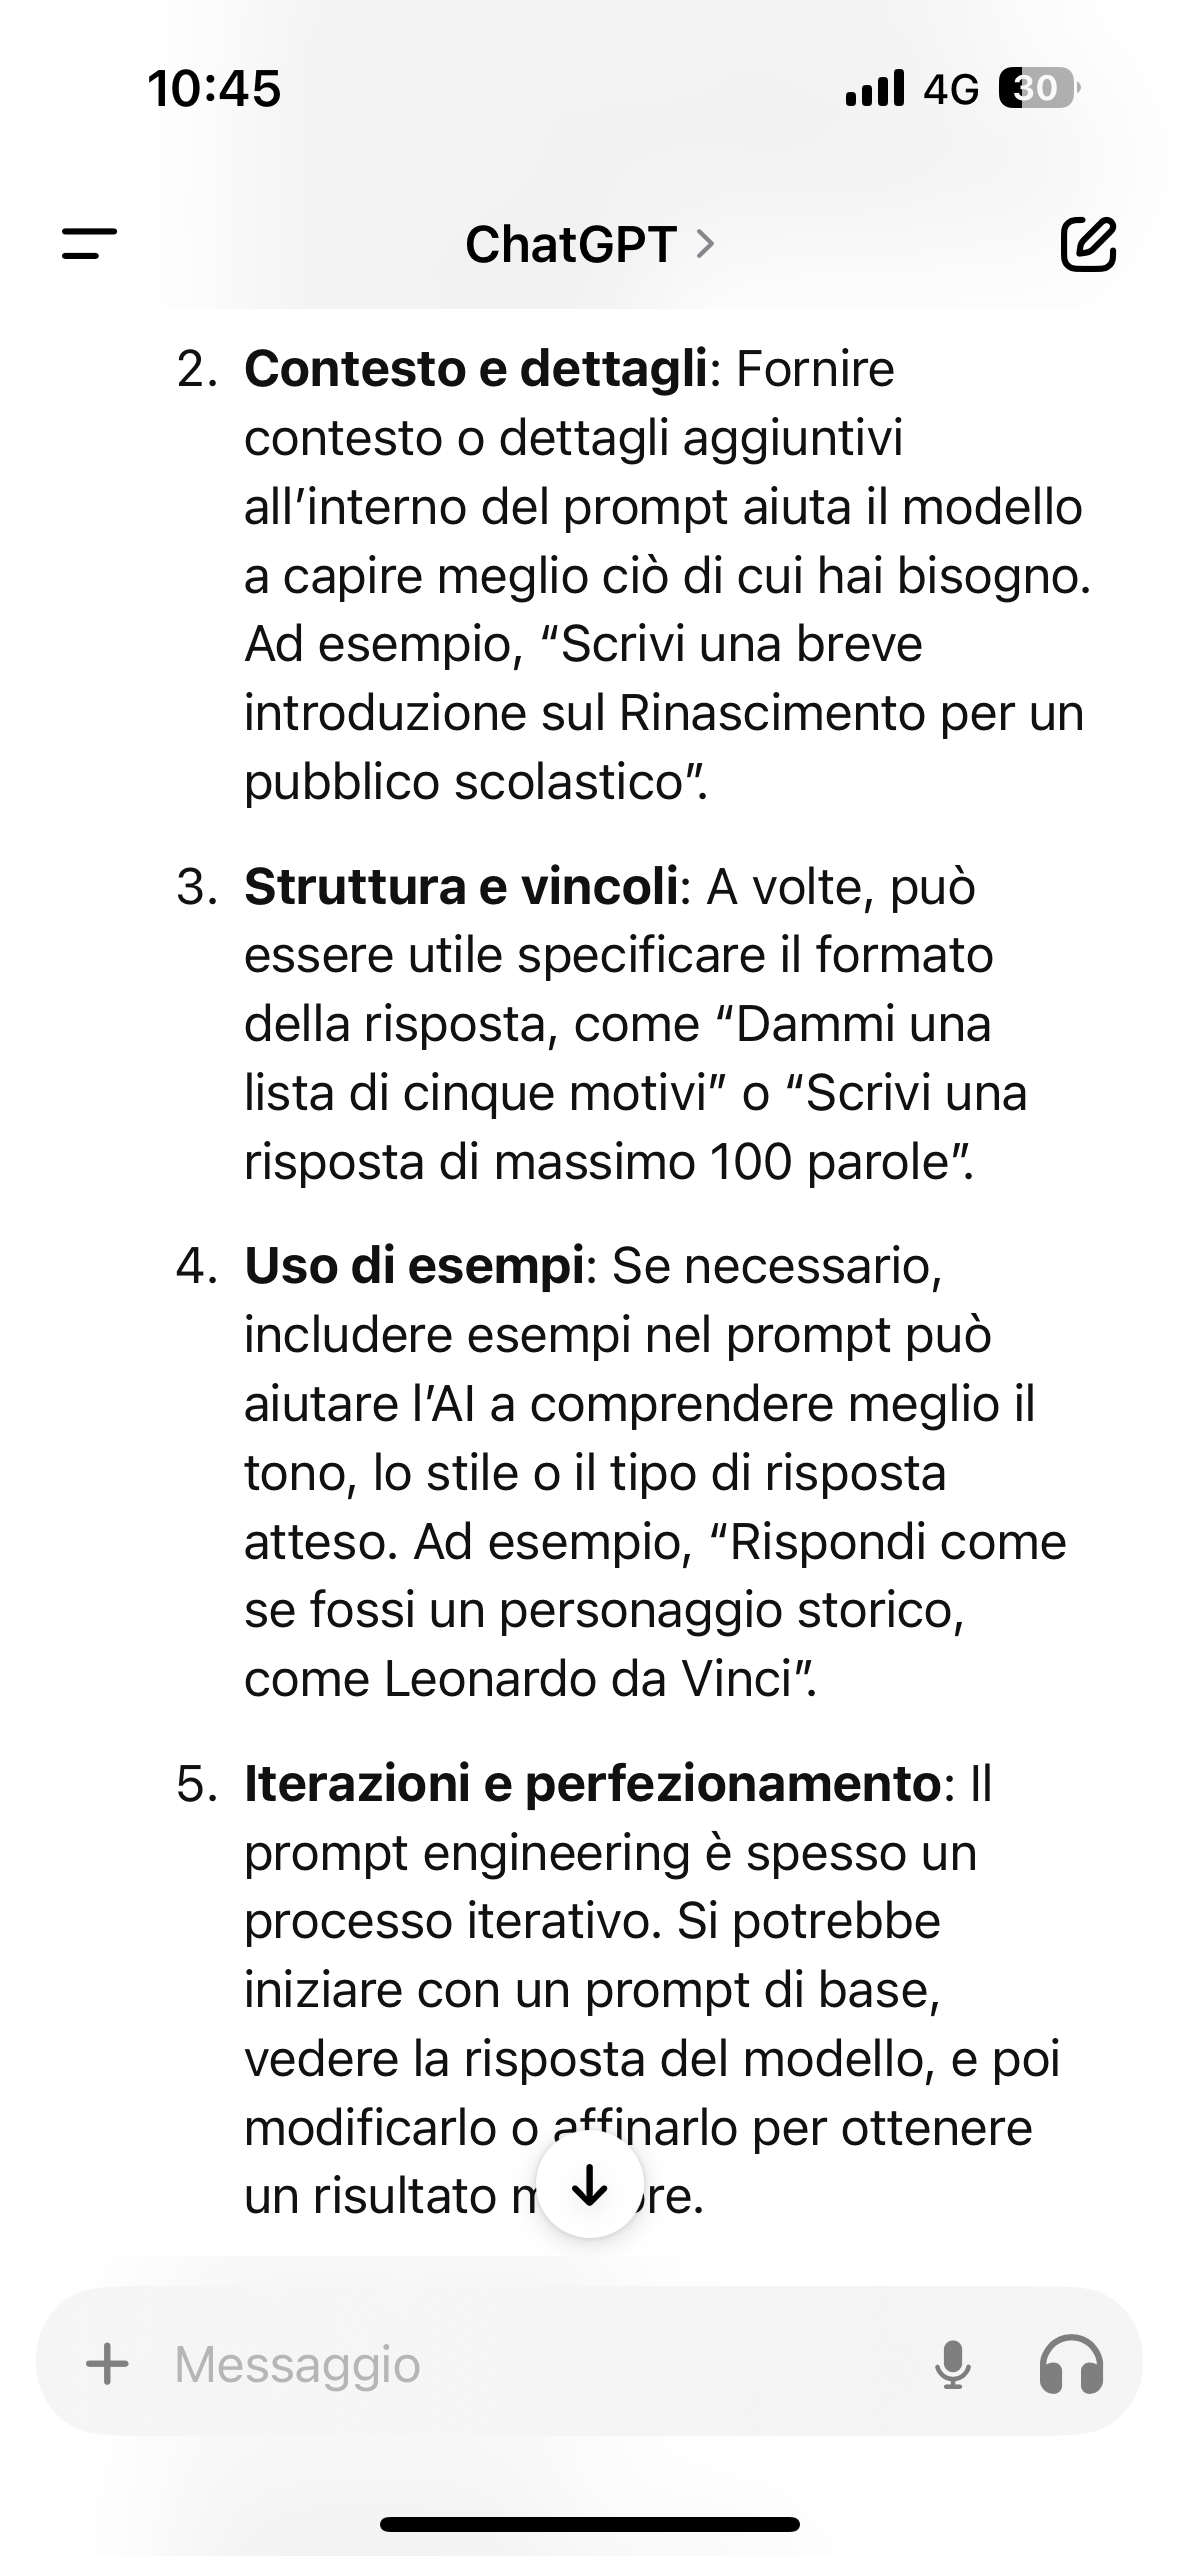
\includegraphics[width=.25\textwidth]{img/PE-3.PNG}
        \end{figure}
    \end{minipage}
    \\\vspace*{.3cm}
    \begin{minipage}[t]{\textwidth}
        \begin{itemize}[leftmargin=10pt,align=right]
            \onslide<1->\item[\alert{\faArrowCircleRight}] Definiamo meglio il concetto di \emph{prompt}$\ldots$
        \end{itemize}
    \end{minipage}
}
\end{frame}
%
\begin{frame}[t] \frametitle{\emph{Prompt Engineering}}
\framesubtitle{Componenti principali}
{\small
\onslide<1->
    \begin{minipage}[t]{\textwidth}
        \begin{itemize}[leftmargin=70pt,align=right]
            \onslide<1->\item[\alert{Istruzione}] indicazioni/suggerimenti specifici che si presentano al modello per raggiungere l'azione desiderata (designano la \emph{task} da compiere)
            \onslide<2->\item[\alert{Contesto}] informazioni aggiuntive che possono indirizzare e addestrare il modello in modo che generi risposte migliori, pertinenti e coerenti con l’obiettivo
            \onslide<3->\item[\alert{Dati di \emph{input}}] il testo contenente ciò a cui si è interessati a trovare una risposta
            \onslide<4->\item[\alert{Indicatore di \emph{output}}] la tipologia o il formato che si vuole ottenere nella risposta
        \end{itemize}
        \vspace*{.5cm}
        \begin{itemize}[leftmargin=10pt,align=right]
            \onslide<5->\item[\alert{\faArrowCircleRight}] Dati di \emph{input} obbligatori
            \onslide<6->\item[\alert{\faArrowCircleRight}] Altri dati opzionali
        \end{itemize}
    \end{minipage}
}
\end{frame}
%
\begin{frame}[t] \frametitle{\emph{Prompt Engineering}}
\framesubtitle{Configurazione LLM per \emph{prompting}}
{\footnotesize
    \begin{minipage}[t]{\textwidth}
        \begin{itemize}[leftmargin=80pt,align=right]
            \onslide<1->\item[\alert{Creatività del modello}] quanta libertà lasciamo al LLM nella scelta del \emph{token} successivo
            \begin{itemize}[leftmargin=50pt,align=right]
            \onslide<2->\item[\alert{Temperatura}] più è bassa, più deterministica la generazione dei \emph{token} successivi (ovvero, preso sempre il \emph{token} più probabile)
            \onslide<3->\item[\alert{\emph{Top P}}] definisce una finestra di probabilità entro la quale poter scegliere il \emph{token} successivo (da abbassare quando si vogliono risposte fattuali, da alzare se si vuole un testo più ``fuori dagli schemi'')
            \onslide<4->\item[\alert{\faExclamationTriangle}] Non modificare entrambe!!!
            \end{itemize}
            \onslide<5->\item[\alert{Lunghezza massima}] numero di \emph{token} massimo generato dal modello
            \onslide<6->\item[\alert{\emph{Stop sequences}}] lista di \emph{token} che dice al modello di terminare la generazione
            \onslide<7->\item[\alert{\emph{Token penalties}}] contro la ripetizione dei medesimi \emph{token}
            \begin{itemize}[leftmargin=63pt,align=right]
                \onslide<8->\item[\alert{\emph{Frequence penalty}}] proporzionalmente al n° di volte usato nella sequenza
                \onslide<9->\item[\alert{\emph{Presence penalty}}] globale per tutti i \emph{token} ripetuti
                \onslide<10->\item[\alert{\faExclamationTriangle}] Non modificare entrambe!!!
            \end{itemize}
        \end{itemize}
    \end{minipage}
}
\end{frame}
%
\begin{frame}[t] \frametitle{\emph{Prompt Engineering}}
\framesubtitle{Tipologie di \emph{prompting}}
{\footnotesize
    \begin{minipage}[t]{\textwidth}
        \begin{itemize}[leftmargin=50pt,align=right]
            \onslide<1->\item[\alert{\emph{Direct}}] solo dati di \emph{input}, senza nemmeno definire la \emph{task} obiettivo
            \begin{itemize}[leftmargin=15pt,align=right]
                \item[\alert{\faArrowCircleRight}] Utilizzare il modello secondo la sua natura specifica, senza specializzarlo
            \end{itemize}
            \onslide<2->\item[\alert{\emph{0-Shot}}] \emph{task} specificata, ma la richiesta dell'utente è priva di informazioni sul contesto o priva di esempi
            \onslide<3->\item[\alert{\emph{Few-shots}}] la richiesta dell'utente è seguita da alcuni esempi su cui la LLM tara il \emph{template} delle risposte da fornire
            \onslide<4->\item[\alert{\emph{Role-based}}] le informazioni del \emph{prompt} sono suddivise tra una entità \emph{superuser} (\emph{system} o \emph{admin}) e una entità \emph{user}
            \begin{itemize}[leftmargin=15pt,align=right]
                \onslide<5->\item[\alert{\faArrowCircleRight}] Contesto, definizione \emph{task} e formattazione \emph{output} al \emph{system}
                \onslide<6->\item[\alert{\faArrowCircleRight}] \emph{Input} allo \emph{user}
            \end{itemize}
            \onslide<7->\item[\alert{\emph{Chain-of-Thought}}] il \emph{prompt} viene costruito affinché il LLM possa ``ragionare'' per passi sequenziali, sfruttando man mano i dati che ha generato
            \begin{itemize}[leftmargin=15pt,align=right]
                \onslide<8->\item[\alert{\faArrowCircleRight}] Utilizzato per le \emph{task} di risoluzione problemi di logica, matematica e simili
            \end{itemize}
        \end{itemize}
    \end{minipage}
}
\end{frame}
%